\documentclass[letterpaper, 12pt]{article}

%%%%%%%%%%%%%%%%%%%%%%%%%%%%%
% DEFINITIONS
% Change those informations
% If you need umlauts you have to escape them, e.g. for an ü you have to write \"u
\gdef\mytitle{Systemtechnik - Ausarbeitung}
\gdef\mythema{Quantencomputing}

\gdef\mysubject{Systemtechnik}
\gdef\mycourse{5BHITT 2015/16}
\gdef\myauthor{Klaus Ableitinger\\Sebastian Steinkellner}

\gdef\myversion{0.1}
\gdef\mybegin{26. M\"arz 2016}
\gdef\myfinish{\today}

\gdef\mygrade{Note:}
\gdef\myteacher{Betreuer: Mi. Borko \& Ma. Schabel}
%
%%%%%%%%%%%%%%%%%%%%%%%%%%%%%

%!TEX root=../document.tex

\usepackage[english, ngerman]{babel}
\usepackage[in]{fullpage}
\usepackage{hyperref}
% Fontencoding for possible copy&paste out of PDF
\usepackage[T1]{fontenc}
\usepackage[utf8]{inputenc}
\usepackage{graphicx} 
\usepackage{textcomp}
\usepackage{sectsty}
\usepackage{caption}
\usepackage{listings}
\usepackage{array}
\usepackage{colortbl}
\usepackage{footmisc}
\usepackage{fancyhdr}
\usepackage{ccicons}
\usepackage{suffix}
\usepackage{multirow}
\usepackage{tabularx}
\usepackage{amsmath}
\usepackage{listings}
\usepackage{color}
\usepackage{url}
\usepackage[dvipsnames]{xcolor}
%\usepackage[longnamesfirst,nonamebreak]{natbib}
\usepackage[headsep=1cm,headheight=3cm,hmargin=2cm,vmargin=2.5cm]{geometry}
\usepackage[nolist]{acronym}

% Definitions for Textcolor
\usepackage{color}
\definecolor{listings}{rgb}{0.96, 0.96, 0.96}
\definecolor{update}{rgb}{1, 0.8, 0.8}
\definecolor{config}{rgb}{0.8, 1, 0.8}
\definecolor{gray}{rgb}{0.4,0.4,0.4}
\definecolor{darkblue}{rgb}{0.0,0.0,0.6}
\definecolor{cyan}{rgb}{0.0,0.6,0.6}

% Java Syntaxhighligthning
% strings
\definecolor{javared}{rgb}{0.6,0,0}
% comments
\definecolor{javagreen}{rgb}{0.25,0.5,0.35}
% keywords
\definecolor{javapurple}{rgb}{0.5,0,0.35}
% javadoc
\definecolor{javadocblue}{rgb}{0.25,0.35,0.75}

\lstset{
	basicstyle=\ttfamily\small,
	keywordstyle=\bfseries\color[rgb]{0.496,0.000,0.332},
	commentstyle=\color[rgb]{0.246,0.496,0.371},
	stringstyle=\color[rgb]{0.164,0.000,0.996},
	tabsize=4,
	breaklines=true,
	numbers=left,
	numberstyle=\tiny\color{black},
	stepnumber=5,
	numbersep=10pt,
	numberstyle=\tiny,
	captionpos=b,
	xleftmargin=1cm,
	showspaces=false,
	showstringspaces=false,
	basewidth={0.53em,0.45em},
	frame=single,
	xleftmargin=1cm,
	basicstyle=\scriptsize,
}


\lstdefinestyle{Java}{
	language=Java,
	keywordstyle=\color{javapurple}\bfseries,
	stringstyle=\color{javared},
	commentstyle=\color{javagreen},
	morecomment=[s][\color{javadocblue}]{/**}{*/},
}

\lstdefinestyle{XML}{
	language=XML,
	basicstyle=\ttfamily,
	columns=fullflexible,
	commentstyle=\color{gray}\upshape
}

\lstdefinelanguage{XML}
{
	morestring=[b]",
	morestring=[s]{>}{<},
	morecomment=[s]{<?}{?>},
	stringstyle=\color{black},
	identifierstyle=\color{darkblue},
	keywordstyle=\color{cyan},
	% list your attributes here
	morekeywords={xmlns,version,type}
}


\let\tempsection\section
\renewcommand\section[1]{\vspace{-0.3cm}\tempsection{#1}\vspace{-0.3cm}}
\WithSuffix\newcommand\section*[1]{\tempsection*{#1}}

\let\tempsubsection\subsection
\renewcommand\subsection[1]{\vspace{0cm}\tempsubsection{#1}\vspace{0cm}}

\let\tempsubsubsection\subsubsection
\renewcommand\subsubsection[1]{\vspace{0cm}\tempsubsubsection{#1}\vspace{0cm}}

\linespread{0.94}

\lhead{\mysubject}
\chead{}
\rhead{\bfseries\mythema}
\lfoot{\mycourse}
\cfoot{\thepage}
% Creative Commons license BY
% http://creativecommons.org/licenses/?lang=de
\rfoot{\ccby\hspace{2mm}\myauthor}
\renewcommand{\headrulewidth}{0.4pt}
\renewcommand{\footrulewidth}{0.4pt}

\begin{document}
\parindent 0pt
\parskip 6pt

\pagenumbering{Roman} 
%!TEX root=../laborprotokoll.tex

\begin{titlepage}

	\begin{figure}[!h]
		\begin{flushright}
			
\includegraphics[width=0.3\linewidth]{images/jdIT_tgm.png}
		\end{flushright}
	\end{figure}

	\vspace{2.5cm} 

	{\begin{center} \bfseries\huge
			\rule{17.5cm}{0.1mm}  
			\\[5mm]
			\mytitle\\[5mm]
			\mythema\\
			\rule{17.5cm}{0.1mm}  
	\end{center}}

	{\begin{flushright} \bfseries\Large
			\vspace{2cm}
			\mysubject\\
			\mycourse\\[10mm]
			\myauthor\\[10mm]
	\end{flushright}}

	{\begin{table}[!h] \bfseries\normalsize
		\begin{tabularx}{\textwidth}{lXr @{\hspace{0mm}}}
			&& Version \myversion\\
			\mygrade && Begonnen am \mybegin\\
			\myteacher && Beendet am \myfinish\\
		\end{tabularx}
	\end{table}}

\end{titlepage}


\clearpage
\thispagestyle{empty}
\tableofcontents

\newpage
\pagenumbering{arabic}
\pagestyle{fancy}

%\vspace{-0.5cm}
%%!TEX root=../document.tex

\section{Hardware-Aufbau}
\label{sec:Hardware-Aufbau}


\subsection{Qubit}
\label{sec:Qubit}

\subsubsection{Schrödinger}

Schroedingers Katze ist die berühmteste Veranschaulichung eines grundlegenden Phänomens der Quantenmechanik. Genaugenommen ist es ein Versuchsaufbau, anhand dessen sich verschiedene Begriffe der Quantenmechanik leicht erklären lassen. Der Versuchsaufbau sieht folgendermaßen aus:

In einer Kiste befinden sich eine Katze und eine Ampulle mit einer Giftigen Substanz. Mit einer exakten Wahrscheinlichkeit von 50\% ist die Ampulle offen und die Katze bereits tot, mit einer genau gleich großen Wahrscheinlichkeit ist aber die Ampulle immer noch verschlossen und die Katze am Leben. Da wir nur die Außenseite der Kiste sehen und sie Schall und Geruchdicht ist, können wir nicht genau sagen, in welchem Zustand die Katze sich befindet. Es könnte also behauptet werden, dass sie gleichzeitig tot und lebendig ist.
Den Umstand, dass 2 (oft gegensätzliche) Zustände wahr sind, wird in der Quantenmechanik als Superposition bezeichnet. Eine Vorraussetzung für das erreichen einer Superposition ist die vollkommene Abschottung von der Außenwelt. 

Wenn nun die Kiste geöffnet wird und der Betrachter einen Blick ins innere der Kiste wirft, so erkennt er ziemlich schnell, ob die Katze tot oder lebendig ist. Einer der Beiden Zustände ist durch diese sogenannte Messung verloren gegangen.

\subsubsection{Definition}

Per Definition werden die Zustände eines Quantenbits in der Form $\alpha * |0\rangle + \beta * |1\rangle$ angeschrieben.
$\alpha$ und $\beta$ werden ''Amplituden'' genannt, sind komplexe Zahlen und durch die Formel $|\alpha|^2 + |\beta|^2 = 1$ voneinander abhängig.
Anders als ein klassisches Bit, kann ein Qubit nicht gelesen, sondern muss gemessen werden, wobei die Superposition zerstört wird und anhand der Amplituden (die einen Anteil darstellen) folgendermaßen berechnet werden kann, mit welcher Wahrscheinlichkeit sich das Qubit in welchem Zustand befindet: $P(|0\rangle) = |\alpha|^2, P(|1\rangle) = |\beta|^2$

\subsubsection{Messung}

Die Messung erfolgt je nach Ausführung des Quantenbits, da es auf mehrere Arten realisiert werden kann. Wenn Licht eine Rolle spielt, kann die Lichtstärke gemessen werden, wobei diese Art von Qubits nur kürzer als 1 Minuten gespeichert werden kann. Kernspinquantenbits können durch Messung der Magnetfelder, Ionenfallen mithilfe eines Lasers ausgelesen werden. Mehr dazu befindet sich im Kapitel Anforderungen.

\subsubsection{Zustände \& Zustandsänderungen}


\subsection{Register}
\label{sec:Register}

\subsubsection{Definition}
(formeln auf seite 28)

Ein Quantenregister besteht aus einer Reihe von 2 bis n Qubits und wird angeschrieben als $R = |x_1\ranlge|x_0\rangle$
Zur Erklärung ist allerdings eine Beschränkung auf das Minumum von 2 Bits sinnvoll.

\subsubsection{Berechnung}

Die Berechnung des Zustands eines Quantenregisters mit 2 Bit sieht folgendermaßen aus:
\begin{itemize}
    \item $|x_0\ranlge = \gamma|0\rangle + \gamma_1\rangle, |x_1\ranlge = \beta|0\rangle + \beta|1\rangle$
    \item $R = |x_1\ranlge|x_0\rangle$
	\item[=] $(\beta_0|0\rangle+\beta_1|1\rangle)(\gamma_0|0\rangle+\gamma_1|1\rangle)$
	\item[=] $\beta_0\gamma_0|0\rangle|0\rangle+\beta_0\gamma_1|0\rangle|1\rangle+\beta_1\gamma_0|1\rangle|0\rangle+\beta_1\gamma_1|1\rangle|1\rangle$
\end{itemize}

Zur Übersichtlichkeit wird angenommen, das
\begin{itemize}
	\item $\alpha_{i,j} = \beta_i\gamma_j$ und
	\item $|x_1\rangle|x_0\rangle = |x_1 x_0\rangle$
\end{itemize}
sowie die Ziffern vom binären ins dezimale Zahlensystem umgerechnet, wodurch folgende Schreibweise zustande kommt:

$R = \alpha_0|0\rangle+\alpha_1|1\rangle+\alpha_2|2\rangle+\alpha_3|3\rangle$

per Definition kann sich ein Quantenregister in Zuständen der Form

$R = \displaystyle\sum_{i=0}^{2^n-1} \alpha_1|i\rangle$

befinden, wobei die Einschränkung der einzelnen Qubits nicht vergessen werden darf, die für ein Register auf folgende Art geschrieben werden kann:

$\displaystyle\sum_{i=0}^{2^n-1}  |\alpha|^2 = 1$

\subsubsection{Zustände}

Der Zustand des Registers kann dann durch Ausmultiplizieren errechnet werden. -formel 4-

\subsubsection{begriffe ''lokal'' und ''unitär''}

\subsection{Gatter}
\label{sec:Gatter}

\subsubsection{CNOT}

CNOT bedeutet ausgesprochen ''Controlled Not'', was als ''Kontrollierbare Negierungsschaltung'' übersetzt werden kann.
Ein CNOT hat 2 Eingänge und 2 Ausgänge, wobei der zweite Ausgang den invertierten Wert von 1 ausgibt wird, wenn der erste Eingang auf 1 gesetzt ist.

\subsection{Architektur}
\label{sec:Architektur}

\subsubsection{Anforderungen}

Definition von David Deutsch 1985:
Ein Quantencomputer besteht aus einer Reihe von Quantenbits,
\begin{enumerate}
	\item die in einen Anfangszustand versetzt werden können,
	\item die Information robust speichern,
	\item auf die (universelle) Quantengatter anwendbar sind und
	\item die gemessen werden können.
\end{enumerate}

\subsubsection{(De)kohärenz}

Kohärenz bedeutet Zusammenhängend. Dekohärenz ist ein Phänomen der Quantenphysik, das Kohärenzeigenschaften von Systemen kurzzeitig außer Kraft setzt. Dekohärenzeffekte treten auf, wenn ein geschlossenes System geöffnet wird und mit der Umwelt in Wechselwirkung treten kann, wobei die Zustände beider Systeme irreversibel verändert werden.
Im Beispiel mit der Katze, wäre es eine Tote oder lebende Katze, und der Betrachter, der nun weiß, ob die Katze tot oder lebendig ist.

\subsubsection{Photonen}

Die Physiker Ludwig Mach und Ludwig Zehnder entwickelten unabhängig voneinander beide den selben Versuchsaufbau, der heutzutage Mach-Zender-Inferometer genannt wird. Er besteht aus 4 Spiegeln, wovon 2 halbdurchlässig sind, 2 Messgeräten und einem Streifen Papier.

Wenn ein Lichtstrahl in den Aufbau geschickt wird, so wird er über den ersten Spiegel, der halbdurchlässig ist, geteilt in eine gerade und eine um 90° abgelenkte Bahn gelenkt. Nach einem gewissen Abstand befindet sich auf jeder Bahn einer der "normalen" Spiegel, wodurch das Licht jeweils um 90° gelenkt wird und sich die beiden dann an einer Stelle kreuzen, an der der zweite halbdurchlässige Spiegel montiert wird. In eine Bahn wird ein Blatt Papier gehalten. Durch den halbdurchlässigen Spiegel kommt bei beiden Messgeräten gleich viel Licht an. Wird das Blatt Papier entfernt, so kommt es auf einer Bahn zu konstruktiven überlagerungen zwischen dem letzten Spiegel und dem Messgerät, wodurch bei diesem kein Licht ankommt.

Wenn anstelle eines Lichtstrahles nur einzelne Photonen verwendet werden, zeigt sich der selbe Effekt, obwohl eigentlich keines der Photonen wissen kann, ob der Papierstreifen im Weg ist oder nicht. Und hier kommt wieder die Quantenphysik als Erklärung zum einsatz, da ein Teilchen, wie wir schon wissen, solange es nicht beobachtet wird, in mehreren Zuständen gleichzeitig sein kann. Es kann sich also auf beiden Bahnen gleichzeitig bewegen, bis es gemessen wird, wodurch die Superposition zerstört wird und es nur bei einem Messgerät ankommen kann.

\subsubsection{Kernspinresonanz}

Kernspinresonanz ist der Name für einen phyiskalischen Effekt der in Form von Wechselwirkung zwischen Atomkernen und Magnetfeldern auftritt. Der Spin eines Moleküls kann durch Magnetfelder ausgerichtet werden, was ausgenutzt wird, um Quantenbits abzubilden und zu speichern. Durch unterschiedliche chemische Eigenschaften der Umgebung kann jedes Bit einzeln angesprochen werden. Mithilfe eines Hauptmagnetfeldes kann man die Zustande definieren, zum Beispiel als: $gleiche Ausrichtung = |0\rangle, im rechten Winkel = |1\rangle$;

\subsubsection{Ionenfallen}

Ionenfallen sind dazu da, um elektrisch geladene Moleküle oder Atome durch Magnetfelder an ein und der selben Position zu halten, wodurch mit einem gefangenen Ion bis zu 2 Quantenbits abgebildet werden können. Die abstände zwischen mehreren Ionen liegen im Mikrometerbereich, können durch einen Laser einzeln adressiert werden, aber müssen Temperaturmäßig nahe dem Absoluten gehalten werden um sich nicht gegenseitig abzustoßen.

\section{Interkommunikation}
\label{sec:Interkommunikation}


\subsection{Quantennetzwerke/Kanäle}
\label{sec:Quantennetzwerke/Kanale}

\subsubsection{Generelles Schema eines Telekommunikationssystems}

\subsubsection{Klassische- vs. Quanten-Kommunikationskanäle}

\subsubsection{Photonzählung}

Bei der Photonzälung werden zwischen 2 Standorten mit Sichtkontakt einzelne Photonen vom Sender ausgeschickt und vom Empfänger gezählt. Praktisch getestet wurde es von Harald Weinfurter im Jahr 2007 mit einer Strecke von 144 km, wofür große Teleskope verwendet werden mussten.

\subsection{Quantenteleportation}
\label{sec:Quantenteleportation}

Bei der Quantenteleportation sind 2 Atome an verschiedenen Orten durch Verschränkung verbunden, wodurch bei Anderungen an einer Seite die andere Seite gleichzeitig die selbe Änderung erfährt. Allerdings muss im Vorfeld dieses Qubit an den anderen Ort gebracht werden und zur übertragung noch eine klassische Information ausgetauscht werden, um das Qubit auf die entsprechenden Zustände projizieren zu können. Dadurch ist eine Datenübertragung auf Lichtgeschwindigkeit beschränkt und kann nicht absolut Zeitgleich erfolgen.





%!TEX root=../document.tex

\section{Quantenkryptographie}
\label{sec:Quantenkryptographie}

\subsection{One-Time-Pad}

Das One-Time-Pad ein symmetrisches Verschlüsselungsverfahren und funktioniert über einen Schlüssel welcher folgende Eigenschaften erfüllen muss: \cite{onetimepadwiki}
\begin{itemize}
    \item er ist mindestens so lang wie die Nachricht
    \item er ist gleichverteilt zufällig gewählt
    \item er muss geheim bleiben
    \item er darf nicht wiederverwendet werden, auch nicht teilweise
\end{itemize}

Damit erfüllt ein One-Time-Pad Kerckhoffs’ Prinzip, welches besagt, dass die Sicherheit eines Kryptosystems nicht von der Geheimhaltung des Verschlüsselungsalgorithmus abhängen darf, sondern lediglich von der Geheimhaltung des Schlüssels.\cite{onetimepadwiki}

Es erfüllt daher folgende Kriterien:

\begin{itemize}
    \item Es gibt genauso viele Schlüssel wie mögliche Chiffate
    \item Zu jedem Klartext-Chiffrat-Paar gibt es genau einen Schlüssel, der auf den Klartext angewendet das Chiffrat ergibt
\end{itemize}

Dies bedeuted, dass eine mit einem One-Time-Pad Verschlüsselte Nachricht auch mit beliebig hoher Rechenleistung nicht entschlüsselt werden kann, \cite{cryptintroduction} da auch statistische Methoden, welche bei anderen Verschlüsselungsmethoden dazu verwendet werden können, um die Nachricht zu dechiffrieren, bei einem One-Time-Pad nicht funktionieren.

Beim One-Time-Pad handelt es sich also quasi um ein 'perfektes' Verschlüsselungssystem. 
Das größte Problem des One-Time-Pads ist es allerdings, den geheimen Schlüssel an beide Parteien zu übertragen, ohne, dass dieser abgefangen wird.


\subsection{Quanten-Schlüsselaustausch}
\label{sec:Quanten-Schlusselaustausch}

Als Quanten-Schlüsselaustausch bezeichnet man Verfahren der Quanteninformatik, die Eigenschaften der Quantenmechanik nutzen, um zwei Parteien eine gemeinsame Zufallszahl zur Verfügung zu stellen.
Dies löst nun das größte Problem des One-Time-Pad, nämlich die sichere Übertragung des Schlüssels.
Der Quanten-Schlüsselaustausch hat grundlegend nichts mit Quantencomputern zu tun und benötigt auch keinen um durchgeführt zu werden.
Erste Theorien wurden bereits 1984 aufgestellt und 2004 ein erster Banktransfer über einen durch einen Quanten-Schlüsselaustausch erstellten Schlüssel getätigt. \cite{experiement_qsa}

Der Quanten-Schlüsselaustausch funktioniert durch das ''No-Cloning-Theorem'' nach dem Prinzip, einen Angreifer (Man in the Middle) bei der Schlüsselgenerierung zu erkennen, da eine Messung eines quantenmechanischen Zustandes, immer den Wert verändert.


\subsubsection{Funktionsweise}

Die Informationen werden mittels Photonen übertragen. Photonen können horizontal oder vertikal polarisiert sein (– oder |). Ein horizontal polarisiertes Photon wird von einem vertikalen Filter reflektiert, durch einen horizontalen durchgelassen.
Außerdem können Photonen verschiedenartig diagonal polarisiert sein (/, ''rechtsdiagonal'', oder \textbackslash, ''linksdiagonal''). Diese werden wieder von ihren respektiven Filtern reflektiert, oder durchgelassen.
Daraus ergeben sich nun 2 Basen, die +-Basis (- und |) und die $\times$-Basis (/ und \textbackslash).
Jede Polarisation einer Basis bekommt nun einen anderen binären Wert zugewiesen, wobei die Wahl dabei irrelevant ist, sie muss nur bei beiden Parteien gleich sein. 

\begin{figure}[!htb]
	\centering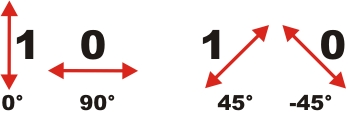
\includegraphics[width=0.6\textwidth]{images/polarisation}
	\caption{Messbasis + (links) und Messbasis $\times$ (rechts) \cite{quantenschluesselaustausch}}
	\label{fig:polarisation}
\end{figure}

Nun beginnt der Sender der Nachricht (Alice), einzelne Photonen an den Empfänger (Bob) zu verschicken. Beide wählen dabei komplett zufällig, mit gleich großer Wahrscheinlichkeit eine Basis aus. 
Alice wählt nun weiters, wieder komplett zufällig und gleichverteilt eine Polarisation aus der ausgewählten Basis und sendet so ein Photon an Bob.

Bob wählt nun auch komplett zufällig und gleichverteilt eine Messbasis aus.
Wenn Bob nun zufällig die gleiche Basis wie Alice verwendet hat, bekommt dieser ein gültiges Ergebnis (also 0 oder 1), wenn er allerdings eine andere Basis verwendet hat wird das gesendete Photon zu 50\% reflektiert oder durchgelassen, ergibt also zu 50\% 0 oder 1, diese Messung ist nicht brauchbar und wird später verworfen.

Nachdem Alice genügend Photonen an Bob geschickt hat, müssen beide Parteien noch bestimmen, welche Messwerte für den Schlüssel verwendet werden sollen.
Dafür machen Alice und Bob die Wahl ihrer Messbasis öffentlich, jedoch nicht welche Polarisation gesendet bzw. empfangen wurde. Sie veröffentlichen also beide eine Liste mit denen von ihnen gewählten Basen (+ oder $\times$).
Schlussendlich vergleichen beide nun diese Listen, wenn sie bei einer Übertragung die gleiche Basis verwendet haben wird der Wert für den Schlüssel verwendet, ansonsten einfach verworfen.
Dadurch werden also ungefähr 50\% der gesendeten bits für die Schlüsselgenerierung verwendet.

\newpage

\begin{table}[ht]
    \centering
    \setlength\tabcolsep{4pt}
    \begin{minipage}{.45\textwidth}
        \centering
        \begin{tabular}{|c|c|c|}
        \hline
        Photon      & Basis     & Bit           \\ \hline
        \textbf{1}  & +         & \textbf{1}    \\ \hline
        2           & $\times$  & 1             \\ \hline 
        \textbf{3}  & +         & \textbf{0}    \\ \hline
        4           & +         & 1             \\ \hline
        \textbf{5}  & $\times$  & \textbf{1}    \\ \hline
        \textbf{6}  & +         & \textbf{0}    \\ \hline
        \textbf{7}  & $\times$  & \textbf{0}    \\ \hline
        8           & $\times$  & 1             \\ \hline
        \end{tabular}
        \caption{Beispielübertragung Alice}
    \end{minipage}%
    \hfill
    \begin{minipage}{.45\textwidth}
        \centering
        \begin{tabular}{|c|c|c|}
        \hline
        Photon      & Basis     & Bit           \\ \hline
        \textbf{1}  & +         & \textbf{1}    \\ \hline
        2           & +         & 0             \\ \hline 
        \textbf{3}  & +         & \textbf{0}    \\ \hline
        4           & $\times$  & 1             \\ \hline
        \textbf{5}  & $\times$  & \textbf{1}    \\ \hline
        \textbf{6}  & +         & \textbf{0}    \\ \hline
        \textbf{7}  & $\times$  & \textbf{0}    \\ \hline
        8           & +         & 0             \\ \hline
        \end{tabular}
        \caption{Beispielmessungen Bob}
    \end{minipage}
\end{table}

In diesem Beispiel sind die \textbf{Fett} hervorgehoben Basen gleich, also wäre der generierte Schlüssel von Alice und Bob 10100; jeweils Photon 1, 3, 5, 6, 7 werden verwendet, die anderen werden verworfen.


\subsubsection{Abhörsicherheit}

Bei dem obigen Verfahren ist es nun auch möglich Abhörsicherheit zu garantieren, sodass eine dritte Person (Eve) sich nich zwischen die Kommunikation schalten und den Schlüsselaustausch abfangen kann.

Um zu versuchen die Kommunikation abzufangen kann Eve sich zwischen Bob und Alice schalten.
Allerdings muss Eve, genauso wie Bob zuerst das gesendete Photon messen und wählt dafür eine zufällige Basis.
Eve muss allerdings sofort wieder ein neues Photon an Bob senden, in 50\% der Fälle wählt Eve zur Messung jedoch die falsche Basis und sendet dadurch ein falsches bit an Bob.
Diesen durch Eve verursachten Fehler können Alice und Bob nun bemerken, wenn sie die gleiche Basis gewählt haben, da sie bei gleicher Wahl immer eindeutige Ergebnisse erhalten sollten.
Außerdem kann Eve so nie den kompletten Schlüssel bekommen, da sie das bit an einer Stelle bei der sie eine falsche Basis verwendet hat, nicht herausfinden kann.

\begin{table}[ht]
    \centering
    \begin{tabular}{|c|c|c|c|c|}
    \hline
    Basis Alice/Bob     & Basis Eve & Empfang Bob   & Übereinstimmung Alice und Bob \\ \hline
    +~+                 & +         & Eindeutig     & 100\% \\ \hline
    +~+                 & $\times$  & Zufall        & 50\%  \\ \hline 
    $\times$~$\times$   & +         & Eindeutig     & 50\%  \\ \hline
    $\times$~$\times$   & $\times$  & Zufall        & 100\% \\ \hline
    
    \end{tabular}
    \caption{Möglichkeiten der Übertragung mit Eve als Man-in-the-Middle \cite{quantenschluesselaustausch}}
    \label{table:eve-moeglichkeiten}
\end{table}

Insgesamt gibt es, wenn Alice und Bob die gleiche Basis gewählt haben, in 25\% der Fällen falsche Messergebnisse. 
Um Eve also zu entdecken müssen Bob und Alice nach der erfolgreichen Übertragung einen Abgleich von einigen (nicht allen!) Werten, bei denen sie die gleiche Basis verwendet haben durchführen, gibt es dort über 25\% Diskrepanz zwischen den Werten, ist sehr Wahrscheinlich ein Man-in-the-Middle Angriff durchgeführt worden.


\subsection{Post-Quanten-Kryptographie}
\label{sec:Post-Quanten-Kryptographie}

Ein besonderer Teil der Quantenkryptographie stellt die Post-Quanten-Kryptographie dar.
Diese behandelt sich mit der Tatsache, dass alle modernen asymmetrischen Verschlüsselungsverfahren durch die Entwicklung eines Quantencomputers unbrauchbar werden.

Die Sicherheit der momentanen Verschlüsselungsverfahren basiert auf den 3 komplizierten mathematischen Problemen:

\begin{itemize}
    \item Faktorisierungsproblem
    \item Diskreter-Logarithmus Problem
    \item Elliptic Curve Cryptography Problem
\end{itemize}

Die obigen Probleme können durch einen Quantencomputer mit Shor's Algorithms innerhalb kürzester Zeit gelöst werden. (siehe \ref{sec:Shor's Algorithmus}).

Damit also momentane Kommunikation auch in Zukunft nicht entschlüsselt werden kann, benötigt man auch jetzt schon Verschlüsselungsverfahren, welche auch Quantencomputer nicht knacken können. \cite{postquantumwiki}


\subsubsection{Post-Quanten-Verschlüsselungsalgorithmen}
\label{sec:Post-Quanten-Verschluesselungsalgorithmen}

Die aktuelle Post-Quanten-Kryptographie Forschung fokussiert sich auf 6 Bereiche: \cite{postquantumwiki}

\begin{itemize}
    \item \textbf{Lattice-based cryptography}
    \item \textbf{Multivariate cryptography}
    \item \textbf{Hash-based cryptography}
    \item \textbf{Code-based cryptography}
    \item \textbf{Supersingular elliptic curve isogeny cryptography}
    \item \textbf{Symmetric key quantum resistance}
\end{itemize}


\subsubsection{Symmetrische Schlüssel Resistenz}
\label{Symmetrische Schlüssel Resistenz}

Symmetrische Schlüssel mit ausreichender Länge, sind bereits heute immun gegen Angriffe von Quantencomputern. \cite{symkeyresistance} 
Zwar können Quantencomputer auch effektivere Brute-Force Angriffe auf einen symmetrischen Schlüssel durchführen, allerdings wird dieser nicht exponentiell schneller, wie bei der asymmetrischen Verschlüsselung.
Darum reicht es einfach, die Schlüssellange zu erhöhen.

\newpage


\section{Quantenalgorithmik}
\label{sec:Quantenalgorithmik}


\subsection{Besonderheiten und Unterschiede zu ''klassischer'' Algorithmik}
\label{sec:Besonderheiten und Unterschiede zu klassischer Algorithmik}

Ein ''klassischer'' (nicht quanten) Algorithmus ist eine endliche Sequenz von Maschineninstruktionen, wo jede Instruktion auf einem klassischen Computer ausgeführt wird.
Ähnlich sind Quantenalgorithmen eine endliche Sequenz von Quanteninstruktionen, welche auf einem Quantencomputer ausgeführt werden. Jedoch kann ein Quantencomputer auch klassische Algorithmen ausführen. \cite{quantenalgorithmgwiki}

Die Besonderheiten von Quantenalgorithmen liegen in der Verwendung von Qubits (siehe \ref{sec:Qubit}), welche quantenmechnische Prinzipien wie die Quantenteleportation und die Superposition verwenden.
Zwar gibt es bereits einige entwickelte Quantenalgorithmen, allerdings ist dieses Gebiet noch nicht sehr gut erforscht.


\subsection{Quantenalgorithmik Übersicht}
\label{sec:Quantenalgorithmik Übersicht}


\subsubsection{Deutsch-Josza Algorithmus}

Dieser Algorithmus kann zum Lösen sogenannter Blackbox-Probleme verwendet werden, für die normale Computer exponentiell viele Zugriffe, ein Quantencomputer allerdings nur einen bräuchte.
Hierbei wird z.B. das Ergebnis einer Funktion $f$ darauf überprüft, ob alle Eingaben konstant 0 als Ergebnis liefern, oder ob beispielsweise die eine Hälfte 0 und die andere Hälfte 1 liefert. \cite{quantenalgorithmgwiki}


\subsubsection{Simons's Algorithmus}

Dieser Algorithmus dient auch zur exponentiell schnelleren Lösung von Blackbox-Problemen und war Vorbild für Shor's Algorithmus. \cite{quantenalgorithmgwiki}

\subsubsection{Quanten Phasen Näherungs-Algorithmus}

Aus der englischen Wikipedia: \cite{quantenalgorithmgwiki}
\begin{quote}
    \textit{The quantum phase estimation algorithm is used to determine the eigenphase of an eigenvector of a unitary gate given a quantum state proportional to the eigenvector and access to the gate.}
\end{quote}
Der Algorithmus wird außerdem oft als Unterfunktion in anderen Quantenalgorithmen verwendet. 


\subsection{Shor's Algorithmus}
\label{sec:Shor's Algorithmus}

Shor's Algorithmus ist ein Quantenmechanischer Algorithmus aus dem mathematischen Gebiet der Zahlentheorie.
Er dient dabei zur Ermittlung eines nicht trivialen Teilers und zählt damit zu den Faktorisierungsalgorithmen.
Für die Faktorisierung einer Zahl $n$ benötigt ein Quantencomputer mindestens $\log{n}$ Qubits.

\newpage

Shor's Algorithmus hat folgende Eigenschaften: \cite{shorwiki}

\begin{itemize}
    \item Eingabe:  zusammengesetzte Zahl $n$
    \item Ausgabe:  ein nicht trivialer Faktor von $n$
    \item Laufzeit: $O((\log{n})^3)$ Gatteroperationen 
\end{itemize}

Shor's Algorithmus läuft also in polynomieller Zeit und ist dem besten bis jetzt bekannten klassischen Faktorisierungsalgorithmus, dem Zahlkörpersieb, welches mit sub-exponentieller Zeit läuft weit überlegen.
Der Zahlenkörpersieb Algorithmus hat eine ungefähre Laufzeit von $O(e^{1.9 (\log{N})^{1/3} (\log{\log{N}})^{2/3}})$. \cite{numberfieldsieve}


Shor's Algorithmus kann man Grundlegend in 2 Teile teilen: einen Klassischen- und einen Quantenteil.
Der Klassische Teil wird zur Reduzierung des Problems verwendet, der Quantenteil dient dann zu effektiven Lösung des Restproblems.


\subsection{Grover's Algorithmus}
\label{sec:Grover's Algorithmus}

Grover's Algorithmus ist ein Quantenalgorithmus zur Suche in einer unsortierten Datenbank mit $N$ Einträgen. Er löst dabei das Problem mit $O(\sqrt{N})$ Schritten und $O(\log N)$ Speicherbedarf.

Die prinzipiell schnellstmögliche Suche in einer unsortierten Datenbank auf einem klassischen Computer, die Linearsuche benötigt dabei $O(N)$ Rechenschritte.
Durch Grover's Algorithmus ergibt sich eine beträchtliche quadratische Beschleunigung gegenüber der Linearsuche.


\subsection{Quanten Programmierung}
\label{sec:Quanten Programmierung}

Es gibt bereits einige Quantenprogrammierprachen, welche bereits zum Ausdruck von Quantenalgorithmen verwendet werden können.
Diese können grob in 2 Gruppen von Quantenprogrammiersprachen eingeteilt werden: Imperative und Funktionale.

Die 2 bekanntesten der ersten Gruppe sind QCL \cite{qcl} und LanQ \cite{lanq}.


\subsubsection{QCL - Quantum computing language}
\label{sec:QCL - Quantum computing language}

QCL ist eine Erweiterung von C; Die Syntax ist identisch mit der von C, mit einigen Quantenmechnanischen Erweiterungen.
Außerdem kann ''klassischer'' und quanten - Code in einem Programm zusammen verwendet werden.

Der grundlegendste quanten-Datentyp in QCL ist das qureg (Quanten Register).
Es ist quasi ein Array von qubits: \cite{quantenprogwiki}

\begin{lstlisting}
qureg x1[2]; // 2-qubit quantum register x1
qureg x2[2]; // 2-qubit quantum register x2
H(x1);       // Hadamard operation on x1
H(x2[1]);    // Hadamard operation on the first qubit of the register x2
\end{lstlisting}

\newpage

Außerdem kann, da die Quantenoperationen nur simuliert werden, der Status des Programms abgerufen werden: \cite{quantenprogwiki}

\begin{lstlisting}
qcl> dump
: STATE: 4 / 32 qubits allocated, 28 / 32 qubits free
0.35355 |0> + 0.35355 |1> + 0.35355 |2> + 0.35355 |3>
+ 0.35355 |8> + 0.35355 |9> + 0.35355 |10> + 0.35355 |11>
\end{lstlisting}

Eine der wichtigsten Funktionen der Sprache ist die Möglichkeit Operationen und Funktionen zu definieren, mit denen Quanteninformation manipuliert werden können.
Zum Beispiel: \cite{quantenprogwiki}

\begin{lstlisting}
operator diffuse (qureg q) {
    H(q);                 // Hadamard Transform
    Not(q);               // Invert q
    CPhase(pi, q);        // Rotate if q=1111..
    !Not(q);              // undo inversion
    !H(q);                // undo Hadamard Transform
}
\end{lstlisting}


\clearpage

\begin{thebibliography}{9}

\bibitem{quanteninformatik}
    Gilbert Brands,
    \emph{Einführung in die Quanteninformatik: Quantenkryptografie, Teleportation und Quantencomputing},
    2011,
    ISBN 9783642206474.
    
\bibitem{experiement_qsa}
    Anton Zeilinger,
    \emph{Bank Transfer via Quantum Cryptography Based on Entangled Photons}, 
    2004, 
    online: \url{https://web.archive.org/web/20150211032846/http://www.secoqc.net/downloads/pressrelease/Banktransfer_english.pdf};
    zuletzt abgerufen 28. März 2016.
    
\bibitem{quantenschluesselaustausch}
    Artikel mit Interaktiven Experimenten zu \emph{Quanten Schlüsselaustausch},
    \url{http://www.didaktik.physik.uni-erlangen.de/quantumlab/};
    zuletzt abgerufen 28. März 2016.
    
\bibitem{quantencomputervideo}
    Video über Basics von Quantencomputern
    \url{https://www.youtube.com/watch?v=JhHMJCUmq28};
    zuletzt abgerufen 28. März 2016.
    
\bibitem{ontetimepadwiki}
    Wikipediaartikel zu \emph{One-Time-Pad},
    \url{https://de.wikipedia.org/wiki/One-Time-Pad};
    zuletzt abgerufen 28. März 2016.
    
\bibitem{kryptwiki}
    Wikipediaartikel zu \emph{Quantenkryptographie},
    \url{https://en.wikipedia.org/wiki/Quantum_cryptography};
    zuletzt abgerufen 28. März 2016.
    
\bibitem{postquantumwiki}
    Wikipediaartikel zu \emph{Post-Quanten-Kryptographie},
    \url{https://de.wikipedia.org/wiki/Post-Quanten-Kryptographie};
    zuletzt abgerufen 28. März 2016.
    
\bibitem{quantenalgorithmgwiki}
    Wikipediaartikel zu \emph{Quantenalgorithmen},
    \url{https://en.wikipedia.org/wiki/Quantum_algorithm};
    zuletzt abgerufen 28. März 2016.

\end{thebibliography}

\listoffigures

\end{document}
